本アプリの依頼側、配達側、店舗側そして管理側の各機能設計について記述する。
\subsection{機能概要図}
以下に示す図は本アプリの機能概要である。

\subsubsection{ログイン関連機能}
図\ref{fig:ログイン関連機能}は、ログイン関連機能の概要図である。
\begin{figure}[H]
  \centering
  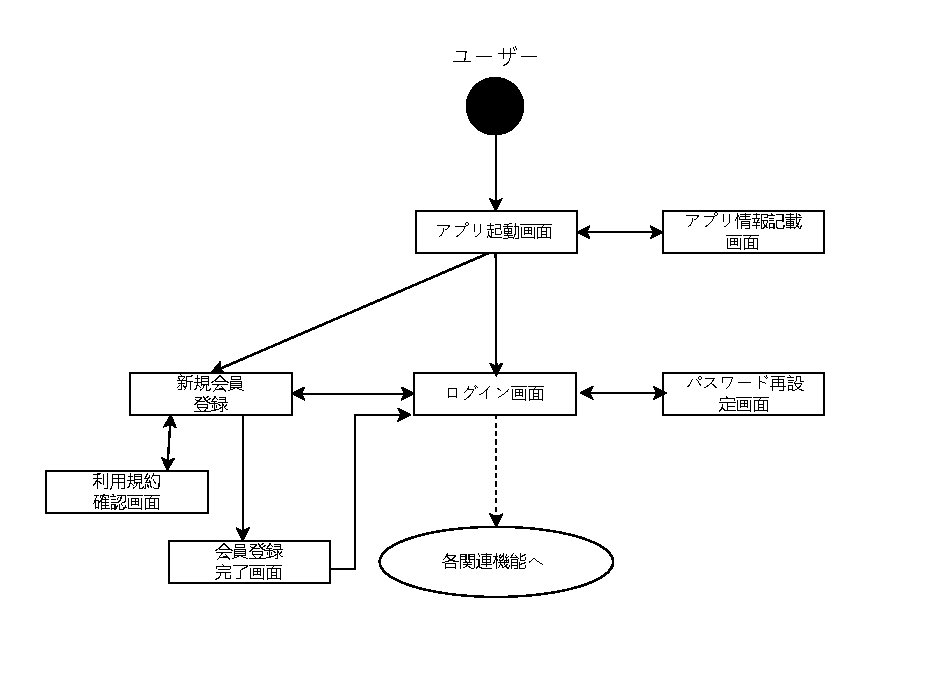
\includegraphics[width=0.75\textwidth]{./ログイン関連機能.pdf}
  \caption{ログイン関連機能}
  \label{fig:ログイン関連機能}
\end{figure}



\subsection{共通機能}
本アプリの依頼側、配達側、店舗側そして管理側の共通の機能設計を以下に記述する。
\subsubsection{新規会員登録機能}
依頼側と配達側、店舗側が利用規約に同意し、情報を入力し、その情報に不備がなく、送信されたメールで本人確認を行うこ
とで、新規会員登録ができる機能である。また、入力情報として、配達側と依頼側は名前、性別、歳、住所、メールアドレス
、電話番号、パスワード、パスワード(確認)を、店舗側は店舗所在地、飲食店営業許可書のファイルおよび写真、メールア
ドレスまたは電話番号、パスワード、パスワード(確認)を入力する。

\begin{figure}[H]
  \centering
  \includegraphics[width=0.75\textwidth]{./新規会員登録機能.pdf}
  \caption{新規会員登録機能}
  \label{fig:新規会員登録機能}
\end{figure}

\subsubsection{ログイン}
アプリ起動時に会員登録済みの利用者(依頼側、配達側、店舗側そして管理側)が、自身のログイン情報を入力することで、
アプリのサービスを利用できるようにする機能である。依頼側、配達側、店舗側はメールアドレスとパスワードを、管理側は
管理者IDとパスワードを入力して、ログインする。

\begin{figure}[H]
  \centering
  \includegraphics[width=0.75\textwidth]{./ログイン.pdf}
  \caption{ログイン機能}
  \label{fig:ログイン}
\end{figure}

\subsubsection{ログアウト}
ログアウトを選択することで、ログイン前の状態に戻す機能で、ログイン画面に遷移する。

\begin{figure}[H]
  \centering
  \includegraphics[width=0.75\textwidth]{./ログアウト.pdf}
  \caption{ログアウト機能}
  \label{fig:ログアウト}
\end{figure}

\subsubsection{退会}
会員が任意のタイミングでアプリ会員から退会する機能。会員情報をデータベースから完全に削除する。

\begin{figure}[H]
  \centering
  \includegraphics[width=0.75\textwidth]{./退会.pdf}
  \caption{退会機能}
  \label{fig:退会}
\end{figure}

\subsubsection{パスワード再発行}
ユーザーはパスワードを忘れた場合、メールアドレスをフォームに入力することで再発行を行う。間違っている場
合はエラーメッセージを出力し、合っている場合はパスワードを生成してデータベースを更新し、メールアドレス宛にそのパス
ワードを送信し、通知画面を表示する。

\begin{figure}[H]
  \centering
  \includegraphics[width=0.75\textwidth]{./パスワード再発行.pdf}
  \caption{パスワード再発行機能}
  \label{fig:パスワード再発行}
\end{figure}

\subsubsection{会員情報確認・変更}
会員がアプリ内のホームページ画面から自身の会員情報を確認・変更するための機能である。

\begin{figure}[H]
  \centering
  \includegraphics[width=0.75\textwidth]{./会員情報確認変更.pdf}
  \caption{会員情報確認・変更}
  \label{fig:会員情報確認変更}
\end{figure}

\subsubsection{会員情報確認・変更}
会員がアプリの操作方法などの問い合わせを管理者に対して行うための機能である。
問い合わせへの回答は会員登録したメールアドレスに送信される。

\begin{figure}[H]
  \centering
  \includegraphics[width=0.75\textwidth]{./問い合わせ機能.pdf}
  \caption{問い合わせ機能}
  \label{fig:問い合わせ機能}
\end{figure}

\subsection{依頼側}



\subsection{配達側}

\subsection{店舗側}

\subsection{管理側}

